\documentclass{article}\usepackage[]{graphicx}\usepackage[]{color}
% maxwidth is the original width if it is less than linewidth
% otherwise use linewidth (to make sure the graphics do not exceed the margin)
\makeatletter
\def\maxwidth{ %
  \ifdim\Gin@nat@width>\linewidth
    \linewidth
  \else
    \Gin@nat@width
  \fi
}
\makeatother

\definecolor{fgcolor}{rgb}{0.345, 0.345, 0.345}
\newcommand{\hlnum}[1]{\textcolor[rgb]{0.686,0.059,0.569}{#1}}%
\newcommand{\hlstr}[1]{\textcolor[rgb]{0.192,0.494,0.8}{#1}}%
\newcommand{\hlcom}[1]{\textcolor[rgb]{0.678,0.584,0.686}{\textit{#1}}}%
\newcommand{\hlopt}[1]{\textcolor[rgb]{0,0,0}{#1}}%
\newcommand{\hlstd}[1]{\textcolor[rgb]{0.345,0.345,0.345}{#1}}%
\newcommand{\hlkwa}[1]{\textcolor[rgb]{0.161,0.373,0.58}{\textbf{#1}}}%
\newcommand{\hlkwb}[1]{\textcolor[rgb]{0.69,0.353,0.396}{#1}}%
\newcommand{\hlkwc}[1]{\textcolor[rgb]{0.333,0.667,0.333}{#1}}%
\newcommand{\hlkwd}[1]{\textcolor[rgb]{0.737,0.353,0.396}{\textbf{#1}}}%
\let\hlipl\hlkwb

\usepackage{framed}
\makeatletter
\newenvironment{kframe}{%
 \def\at@end@of@kframe{}%
 \ifinner\ifhmode%
  \def\at@end@of@kframe{\end{minipage}}%
  \begin{minipage}{\columnwidth}%
 \fi\fi%
 \def\FrameCommand##1{\hskip\@totalleftmargin \hskip-\fboxsep
 \colorbox{shadecolor}{##1}\hskip-\fboxsep
     % There is no \\@totalrightmargin, so:
     \hskip-\linewidth \hskip-\@totalleftmargin \hskip\columnwidth}%
 \MakeFramed {\advance\hsize-\width
   \@totalleftmargin\z@ \linewidth\hsize
   \@setminipage}}%
 {\par\unskip\endMakeFramed%
 \at@end@of@kframe}
\makeatother

\definecolor{shadecolor}{rgb}{.97, .97, .97}
\definecolor{messagecolor}{rgb}{0, 0, 0}
\definecolor{warningcolor}{rgb}{1, 0, 1}
\definecolor{errorcolor}{rgb}{1, 0, 0}
\newenvironment{knitrout}{}{} % an empty environment to be redefined in TeX

\usepackage{alltt}
\usepackage[sc]{mathpazo}
\renewcommand{\sfdefault}{lmss}
\renewcommand{\ttdefault}{lmtt}
\usepackage[T1]{fontenc}
\usepackage{geometry}
\geometry{verbose,tmargin=2.5cm,bmargin=2.5cm,lmargin=2.5cm,rmargin=2.5cm}
\setcounter{secnumdepth}{2}
\setcounter{tocdepth}{2}
\usepackage[unicode=true,pdfusetitle,
 bookmarks=true,bookmarksnumbered=true,bookmarksopen=true,bookmarksopenlevel=2,
 breaklinks=false,pdfborder={0 0 1},backref=false,colorlinks=false]
 {hyperref}
\hypersetup{
 pdfstartview={XYZ null null 1}}

\makeatletter
%%%%%%%%%%%%%%%%%%%%%%%%%%%%%% User specified LaTeX commands.
\renewcommand{\textfraction}{0.05}
\renewcommand{\topfraction}{0.8}
\renewcommand{\bottomfraction}{0.8}
\renewcommand{\floatpagefraction}{0.75}

\makeatother
\IfFileExists{upquote.sty}{\usepackage{upquote}}{}
\begin{document}








The results below are generated from an R script.

\begin{knitrout}
\definecolor{shadecolor}{rgb}{0.969, 0.969, 0.969}\color{fgcolor}\begin{kframe}
\begin{alltt}
\hlcom{#Analysis Walmart Store Sales}
\hlcom{#Date Created: 30/5/2021}
\hlcom{#Author: Sukanto Mukherjee}

\hlkwd{getwd}\hlstd{()}
\end{alltt}
\begin{verbatim}
## [1] "/Users/sukanto/WD/Walmart_StoreSale_Analysis/Walmart_StoreSales_Analysis"
\end{verbatim}
\begin{alltt}
\hlkwd{setwd}\hlstd{(}\hlstr{'/users/sukanto/WD/Walmart_StoreSale_Analysis/Walmart_StoreSales_Analysis'}\hlstd{)}
\hlkwd{install.packages}\hlstd{(}\hlstr{"fpp2"}\hlstd{)}
\end{alltt}
\begin{verbatim}
## 
## The downloaded binary packages are in
## 	/var/folders/47/61hl1t6x1mq6xtl8jw4tf7fh0000gn/T//Rtmp45xPp2/downloaded_packages
\end{verbatim}
\begin{alltt}
\hlcom{#Installing and loading packages}
\hlstd{my_packages} \hlkwb{<-} \hlkwd{c}\hlstd{(}\hlstr{"ggplot2"}\hlstd{,}\hlstr{"lubridate"}\hlstd{,}\hlstr{"dplyr"}\hlstd{,} \hlstr{"plyr"}\hlstd{,}\hlstr{"ggplot2"}\hlstd{,}
                 \hlstr{"lubridate"}\hlstd{,}\hlstr{"raster"}\hlstd{,}\hlstr{"zoo"}\hlstd{,}\hlstr{"sp"}\hlstd{,}
                 \hlstr{"usdm"}\hlstd{,}\hlstr{"lmtest"}\hlstd{,}\hlstr{"forecast"}\hlstd{)}
\hlkwd{lapply}\hlstd{(my_packages, require,} \hlkwc{character.only} \hlstd{=} \hlnum{TRUE}\hlstd{)}
\end{alltt}
\begin{verbatim}
## [[1]]
## [1] TRUE
## 
## [[2]]
## [1] TRUE
## 
## [[3]]
## [1] TRUE
## 
## [[4]]
## [1] TRUE
## 
## [[5]]
## [1] TRUE
## 
## [[6]]
## [1] TRUE
## 
## [[7]]
## [1] TRUE
## 
## [[8]]
## [1] TRUE
## 
## [[9]]
## [1] TRUE
## 
## [[10]]
## [1] TRUE
## 
## [[11]]
## [1] TRUE
## 
## [[12]]
## [1] TRUE
\end{verbatim}
\begin{alltt}
\hlstd{stores} \hlkwb{<-} \hlkwd{read.csv}\hlstd{(}\hlstr{'Walmart_Store_sales.csv'}\hlstd{)}
\hlkwd{head}\hlstd{(stores)}
\end{alltt}
\begin{verbatim}
##   Store       Date Weekly_Sales Holiday_Flag Temperature Fuel_Price      CPI Unemployment
## 1     1 05-02-2010      1643691            0       42.31      2.572 211.0964        8.106
## 2     1 12-02-2010      1641957            1       38.51      2.548 211.2422        8.106
## 3     1 19-02-2010      1611968            0       39.93      2.514 211.2891        8.106
## 4     1 26-02-2010      1409728            0       46.63      2.561 211.3196        8.106
## 5     1 05-03-2010      1554807            0       46.50      2.625 211.3501        8.106
## 6     1 12-03-2010      1439542            0       57.79      2.667 211.3806        8.106
\end{verbatim}
\begin{alltt}
\hlkwd{summary}\hlstd{(stores)}
\end{alltt}
\begin{verbatim}
##      Store        Date            Weekly_Sales      Holiday_Flag      Temperature    
##  Min.   : 1   Length:6435        Min.   : 209986   Min.   :0.00000   Min.   : -2.06  
##  1st Qu.:12   Class :character   1st Qu.: 553350   1st Qu.:0.00000   1st Qu.: 47.46  
##  Median :23   Mode  :character   Median : 960746   Median :0.00000   Median : 62.67  
##  Mean   :23                      Mean   :1046965   Mean   :0.06993   Mean   : 60.66  
##  3rd Qu.:34                      3rd Qu.:1420159   3rd Qu.:0.00000   3rd Qu.: 74.94  
##  Max.   :45                      Max.   :3818686   Max.   :1.00000   Max.   :100.14  
##    Fuel_Price         CPI         Unemployment   
##  Min.   :2.472   Min.   :126.1   Min.   : 3.879  
##  1st Qu.:2.933   1st Qu.:131.7   1st Qu.: 6.891  
##  Median :3.445   Median :182.6   Median : 7.874  
##  Mean   :3.359   Mean   :171.6   Mean   : 7.999  
##  3rd Qu.:3.735   3rd Qu.:212.7   3rd Qu.: 8.622  
##  Max.   :4.468   Max.   :227.2   Max.   :14.313
\end{verbatim}
\begin{alltt}
\hlkwd{colnames}\hlstd{(stores)}
\end{alltt}
\begin{verbatim}
## [1] "Store"        "Date"         "Weekly_Sales" "Holiday_Flag" "Temperature" 
## [6] "Fuel_Price"   "CPI"          "Unemployment"
\end{verbatim}
\begin{alltt}
\hlkwd{str}\hlstd{(stores)}
\end{alltt}
\begin{verbatim}
## 'data.frame':	6435 obs. of  8 variables:
##  $ Store       : int  1 1 1 1 1 1 1 1 1 1 ...
##  $ Date        : chr  "05-02-2010" "12-02-2010" "19-02-2010" "26-02-2010" ...
##  $ Weekly_Sales: num  1643691 1641957 1611968 1409728 1554807 ...
##  $ Holiday_Flag: int  0 1 0 0 0 0 0 0 0 0 ...
##  $ Temperature : num  42.3 38.5 39.9 46.6 46.5 ...
##  $ Fuel_Price  : num  2.57 2.55 2.51 2.56 2.62 ...
##  $ CPI         : num  211 211 211 211 211 ...
##  $ Unemployment: num  8.11 8.11 8.11 8.11 8.11 ...
\end{verbatim}
\begin{alltt}
\hlcom{#Data preprocessing and Exploratory data analysis}

\hlcom{#sum(is.na(stores))}
\hlcom{#duplicated(stores)}


\hlcom{#Formatting date column}


\hlstd{stores}\hlopt{$}\hlstd{Date} \hlkwb{<-} \hlkwd{as.Date}\hlstd{(stores}\hlopt{$}\hlstd{Date,} \hlkwc{format} \hlstd{=} \hlkwd{c}\hlstd{(}\hlstr{"%m-%d-%Y"}\hlstd{))}
\hlkwd{str}\hlstd{(stores)}
\end{alltt}
\begin{verbatim}
## 'data.frame':	6435 obs. of  8 variables:
##  $ Store       : int  1 1 1 1 1 1 1 1 1 1 ...
##  $ Date        : Date, format: "2010-05-02" "2010-12-02" ...
##  $ Weekly_Sales: num  1643691 1641957 1611968 1409728 1554807 ...
##  $ Holiday_Flag: int  0 1 0 0 0 0 0 0 0 0 ...
##  $ Temperature : num  42.3 38.5 39.9 46.6 46.5 ...
##  $ Fuel_Price  : num  2.57 2.55 2.51 2.56 2.62 ...
##  $ CPI         : num  211 211 211 211 211 ...
##  $ Unemployment: num  8.11 8.11 8.11 8.11 8.11 ...
\end{verbatim}
\begin{alltt}
\hlcom{#Which store had maximum sales?}
\hlstd{each_store} \hlkwb{<-} \hlkwd{aggregate}\hlstd{(Weekly_Sales} \hlopt{~} \hlstd{Store, stores,sum)}
\hlstd{each_store} \hlkwb{<-} \hlkwd{arrange}\hlstd{(each_store,} \hlkwd{desc}\hlstd{(Weekly_Sales))}
\hlkwd{max}\hlstd{(each_store)}
\end{alltt}
\begin{verbatim}
## [1] 301397792
\end{verbatim}
\begin{alltt}
\hlkwd{options}\hlstd{(}\hlkwc{scipen} \hlstd{=} \hlnum{999}\hlstd{)}
\hlkwd{jpeg}\hlstd{(}\hlstr{'max_store_sale.jpg'}\hlstd{)}
\hlkwd{ggplot}\hlstd{(each_store,} \hlkwd{aes}\hlstd{(Store, Weekly_Sales))} \hlopt{+}
  \hlkwd{geom_bar}\hlstd{(}\hlkwc{stat} \hlstd{=} \hlstr{'identity'}\hlstd{,} \hlkwc{color} \hlstd{=} \hlstr{' dark blue'}\hlstd{,}
           \hlkwc{fill} \hlstd{=} \hlstr{' dark blue'}\hlstd{)}
\hlkwd{dev.off}\hlstd{()}
\end{alltt}
\begin{verbatim}
## RStudioGD 
##         2
\end{verbatim}
\begin{alltt}
\hlcom{#Which store had maximum standard deviation and finding coeff of mean to sd}

\hlstd{each_store_sd} \hlkwb{<-} \hlkwd{aggregate}\hlstd{(Weekly_Sales}\hlopt{~}\hlstd{Store,stores, sd)}
\end{alltt}
\end{kframe}

{\centering 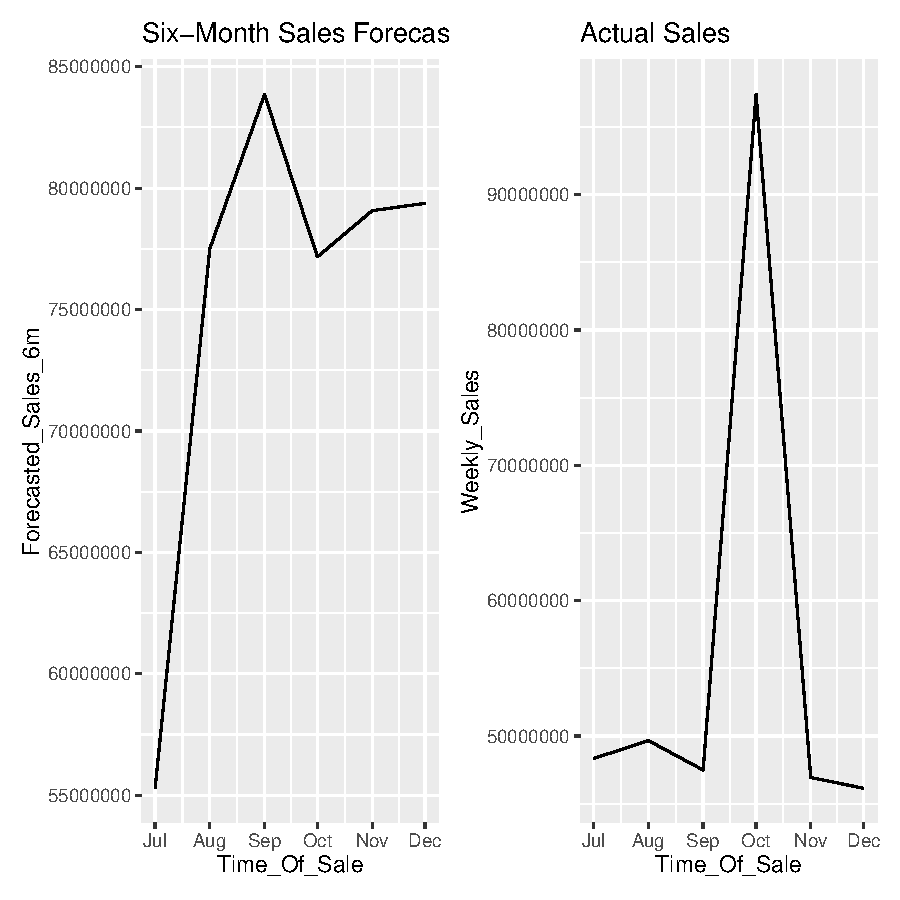
\includegraphics[width=.6\linewidth]{figure/Walmart-Sales-Rnwauto-report-1} 

}


\begin{kframe}\begin{alltt}
\hlstd{each_store_sd} \hlkwb{<-} \hlkwd{rename}\hlstd{(each_store_sd,} \hlkwd{c}\hlstd{(}\hlkwc{Weekly_Sales} \hlstd{=} \hlstr{'SD_Sales'}\hlstd{))}
\hlkwd{max}\hlstd{(each_store_sd)}
\end{alltt}
\begin{verbatim}
## [1] 317569.9
\end{verbatim}
\begin{alltt}
\hlstd{each_store_mean} \hlkwb{<-} \hlkwd{aggregate}\hlstd{(Weekly_Sales}\hlopt{~}\hlstd{Store, stores, mean)}
\hlstd{each_store_mean} \hlkwb{<-} \hlkwd{rename}\hlstd{(each_store_mean,} \hlkwd{c}\hlstd{(}\hlkwc{Weekly_Sales} \hlstd{=} \hlstr{'Mean_Sales'}\hlstd{))}
\hlstd{each_store_mean_sd} \hlkwb{<-} \hlkwd{cbind}\hlstd{(each_store_mean, each_store_sd)}
\hlstd{each_store_mean_sd_coeff} \hlkwb{<-} \hlkwd{transform}\hlstd{(each_store_mean_sd,} \hlkwc{Coeff} \hlstd{= SD_Sales}\hlopt{/}\hlstd{Mean_Sales)}

\hlcom{#Which store had good quarterly growth rate in Q32012?}

\hlstd{quarter_store} \hlkwb{<-} \hlkwd{transform}\hlstd{(stores,} \hlkwc{Q_Flag}\hlstd{=} \hlkwd{ifelse}\hlstd{((Date}\hlopt{>=}\hlstr{'2012-04-01'} \hlopt{&} \hlstd{Date}\hlopt{<=} \hlstr{'2012-06-30'}\hlstd{),}\hlstr{"Q2_2012"}\hlstd{,}
                                                  \hlkwd{ifelse}\hlstd{((Date}\hlopt{>=}\hlstr{'2012-07-01'} \hlopt{&} \hlstd{Date}\hlopt{<=} \hlstr{'2012-09-30'}\hlstd{),}\hlstr{"Q3_2012"}\hlstd{,}\hlstr{"-"}\hlstd{)))}
\hlcom{# confirming start and end date for each quarter}
\hlkwd{aggregate}\hlstd{(Date} \hlopt{~} \hlstd{Q_Flag, quarter_store, min)}
\end{alltt}
\begin{verbatim}
##    Q_Flag       Date
## 1       - 2010-01-10
## 2 Q2_2012 2012-04-05
## 3 Q3_2012 2012-07-09
\end{verbatim}
\begin{alltt}
\hlkwd{aggregate}\hlstd{(Date} \hlopt{~} \hlstd{Q_Flag, quarter_store, max)}
\end{alltt}
\begin{verbatim}
##    Q_Flag       Date
## 1       - 2012-12-10
## 2 Q2_2012 2012-06-07
## 3 Q3_2012 2012-09-03
\end{verbatim}
\begin{alltt}
\hlcom{# summarizing and then reshaping}
\hlstd{quarter_store_sum} \hlkwb{<-} \hlkwd{aggregate}\hlstd{(Weekly_Sales}\hlopt{~}\hlstd{Store}\hlopt{+}\hlstd{Q_Flag,quarter_store,sum)}
\hlkwd{str}\hlstd{(quarter_store_sum)}
\end{alltt}
\begin{verbatim}
## 'data.frame':	135 obs. of  3 variables:
##  $ Store       : int  1 2 3 4 5 6 7 8 9 10 ...
##  $ Q_Flag      : chr  "-" "-" "-" "-" ...
##  $ Weekly_Sales: num  77695537 95522445 20053175 101325671 15693302 ...
\end{verbatim}
\begin{alltt}
\hlstd{quarter_store_sum_t} \hlkwb{<-} \hlkwd{reshape}\hlstd{(quarter_store_sum,}\hlkwc{idvar}\hlstd{=}\hlstr{"Store"}\hlstd{,}\hlkwc{timevar} \hlstd{=}\hlstr{'Q_Flag'}\hlstd{,}\hlkwc{direction}\hlstd{=}\hlstr{"wide"}\hlstd{)}
\hlkwd{View}\hlstd{(quarter_store_sum_t)}
\hlstd{quarter_store_sum_t_GR} \hlkwb{<-} \hlkwd{transform}\hlstd{(quarter_store_sum_t,}
                                        \hlkwc{GR}\hlstd{=((Weekly_Sales.Q3_2012}\hlopt{-}\hlstd{Weekly_Sales.Q2_2012)}\hlopt{/}\hlstd{Weekly_Sales.Q2_2012))}
\hlkwd{jpeg}\hlstd{(}\hlstr{'store_growth_q3.jpg'}\hlstd{)}
\hlkwd{ggplot}\hlstd{(quarter_store_sum_t_GR,} \hlkwd{aes}\hlstd{(Store, GR))}\hlopt{+}\hlkwd{geom_bar}\hlstd{(}\hlkwc{stat}\hlstd{=}\hlstr{'identity'}\hlstd{,}
                                                        \hlkwc{color}\hlstd{=}\hlstr{'dark red'}\hlstd{,}
                                                        \hlkwc{fill} \hlstd{=} \hlstr{'dark red'}\hlstd{)}
\hlkwd{dev.off}\hlstd{()}
\end{alltt}
\begin{verbatim}
## RStudioGD 
##         2
\end{verbatim}
\begin{alltt}
\hlcom{####Some holidays have negative impact on sales. Find out holidays which have higher sales than}
\hlcom{#mean sales in non-holiday season for all stores together}

\hlstd{non_holiday_Sales} \hlkwb{<-} \hlkwd{filter}\hlstd{(stores,Holiday_Flag}\hlopt{==}\hlnum{0}\hlstd{)}
\hlkwd{View}\hlstd{(non_holiday_Sales)}
\hlstd{Avg_non_holiday_Sales} \hlkwb{<-} \hlkwd{mean}\hlstd{(non_holiday_Sales}\hlopt{$}\hlstd{Weekly_Sales)}
\hlstd{Declining_Holiday_Sales} \hlkwb{<-} \hlkwd{filter}\hlstd{(stores,Weekly_Sales}\hlopt{>}\hlstd{Avg_non_holiday_Sales} \hlopt{&} \hlstd{Holiday_Flag}\hlopt{==}\hlnum{1}\hlstd{)}
\hlkwd{unique}\hlstd{(Declining_Holiday_Sales}\hlopt{$}\hlstd{Date)}
\end{alltt}
\begin{verbatim}
## [1] "2010-12-02" "2010-10-09" NA           "2011-11-02" "2011-09-09" "2012-10-02"
## [7] "2012-07-09"
\end{verbatim}
\begin{alltt}
\hlcom{### Provide a monthly and semester view of sales in units and give insights}

\hlstd{stores_month_year} \hlkwb{<-} \hlkwd{transform}\hlstd{(stores,}\hlkwc{Year} \hlstd{=}\hlkwd{as.numeric}\hlstd{(}\hlkwd{format}\hlstd{(Date,}\hlstr{"%Y"}\hlstd{))}
                                     \hlstd{,}\hlkwc{Month} \hlstd{=}\hlkwd{as.numeric}\hlstd{(}\hlkwd{format}\hlstd{(Date,}\hlstr{"%m"}\hlstd{)))}
\hlstd{Summarized_View} \hlkwb{<-} \hlkwd{aggregate}\hlstd{(Weekly_Sales}\hlopt{~}\hlstd{Month}\hlopt{+}\hlstd{Year,stores_month_year,sum)}
\hlstd{Insight_data} \hlkwb{<-} \hlkwd{arrange}\hlstd{(Summarized_View,}\hlkwd{desc}\hlstd{(Weekly_Sales))}
\hlkwd{jpeg}\hlstd{(}\hlstr{'month_sale.jpg'}\hlstd{)}
\hlkwd{ggplot}\hlstd{(Insight_data,} \hlkwd{aes}\hlstd{(Month, Weekly_Sales))} \hlopt{+} \hlkwd{geom_bar}\hlstd{(}\hlkwc{stat}\hlstd{=}\hlstr{'identity'}\hlstd{,}
                                                         \hlkwc{fill} \hlstd{=} \hlstr{'navy'}\hlstd{)}
\hlkwd{dev.off}\hlstd{()}
\end{alltt}
\begin{verbatim}
## RStudioGD 
##         2
\end{verbatim}
\begin{alltt}
\hlkwd{jpeg}\hlstd{(}\hlstr{'year_sale.jpg'}\hlstd{)}
\hlkwd{ggplot}\hlstd{(Insight_data,} \hlkwd{aes}\hlstd{(Year, Weekly_Sales))} \hlopt{+} \hlkwd{geom_bar}\hlstd{(}\hlkwc{stat}\hlstd{=}\hlstr{'identity'}\hlstd{,}
                                                          \hlkwc{fill} \hlstd{=} \hlstr{'dark red'}\hlstd{)}
\hlkwd{dev.off}\hlstd{()}
\end{alltt}
\begin{verbatim}
## RStudioGD 
##         2
\end{verbatim}
\begin{alltt}
\hlcom{# we had experienced maximum sales in Dec 2010 and post that it was in June 2012. }

\hlcom{#Sales Forecast }
\hlcom{#Approach 1: Linear Model}

\hlstd{fit} \hlkwb{<-} \hlkwd{lm}\hlstd{(Weekly_Sales} \hlopt{~} \hlstd{Holiday_Flag} \hlopt{+} \hlstd{Temperature} \hlopt{+} \hlstd{Fuel_Price}
          \hlopt{+} \hlstd{CPI} \hlopt{+} \hlstd{Unemployment, stores)}
\hlkwd{summary}\hlstd{(fit)}
\end{alltt}
\begin{verbatim}
## 
## Call:
## lm(formula = Weekly_Sales ~ Holiday_Flag + Temperature + Fuel_Price + 
##     CPI + Unemployment, data = stores)
## 
## Residuals:
##      Min       1Q   Median       3Q      Max 
## -1022429  -478555  -117266   397246  2800620 
## 
## Coefficients:
##               Estimate Std. Error t value             Pr(>|t|)    
## (Intercept)  1726523.4    79763.5  21.646 < 0.0000000000000002 ***
## Holiday_Flag   74891.7    27639.3   2.710              0.00675 ** 
## Temperature     -724.2      400.5  -1.808              0.07060 .  
## Fuel_Price    -10167.9    15762.8  -0.645              0.51891    
## CPI            -1598.9      195.1  -8.194 0.000000000000000302 ***
## Unemployment  -41552.3     3972.7 -10.460 < 0.0000000000000002 ***
## ---
## Signif. codes:  0 '***' 0.001 '**' 0.01 '*' 0.05 '.' 0.1 ' ' 1
## 
## Residual standard error: 557400 on 6429 degrees of freedom
## Multiple R-squared:  0.02544,	Adjusted R-squared:  0.02469 
## F-statistic: 33.57 on 5 and 6429 DF,  p-value: < 0.00000000000000022
\end{verbatim}
\begin{alltt}
\hlcom{#Dropping the insignificant vars ie Temperature and Fuel Price}
\hlstd{fit1} \hlkwb{<-} \hlkwd{lm}\hlstd{(Weekly_Sales} \hlopt{~} \hlstd{Holiday_Flag} \hlopt{+} \hlstd{CPI} \hlopt{+} \hlstd{Unemployment, stores)}
\hlkwd{summary}\hlstd{(fit1)}
\end{alltt}
\begin{verbatim}
## 
## Call:
## lm(formula = Weekly_Sales ~ Holiday_Flag + CPI + Unemployment, 
##     data = stores)
## 
## Residuals:
##      Min       1Q   Median       3Q      Max 
## -1011980  -480010  -114644   392944  2826593 
## 
## Coefficients:
##               Estimate Std. Error t value             Pr(>|t|)    
## (Intercept)  1664939.2    51224.4  32.503 < 0.0000000000000002 ***
## Holiday_Flag   84509.5    27250.4   3.101              0.00194 ** 
## CPI            -1652.8      185.2  -8.923 < 0.0000000000000002 ***
## Unemployment  -42542.2     3886.5 -10.946 < 0.0000000000000002 ***
## ---
## Signif. codes:  0 '***' 0.001 '**' 0.01 '*' 0.05 '.' 0.1 ' ' 1
## 
## Residual standard error: 557500 on 6431 degrees of freedom
## Multiple R-squared:  0.02479,	Adjusted R-squared:  0.02434 
## F-statistic:  54.5 on 3 and 6431 DF,  p-value: < 0.00000000000000022
\end{verbatim}
\begin{alltt}
\hlcom{#The p-values are too low to support any hypothesis with a linear model}

\hlcom{#Approach 2 : Time series model}
\hlcom{# visually identifying if data is fit for time series}
\hlstd{store1} \hlkwb{<-} \hlkwd{aggregate}\hlstd{(Weekly_Sales}\hlopt{~}\hlstd{Date,stores,sum)}
\hlkwd{plot}\hlstd{(store1,} \hlkwc{type} \hlstd{=} \hlstr{'l'}\hlstd{)}
\end{alltt}
\end{kframe}

{\centering 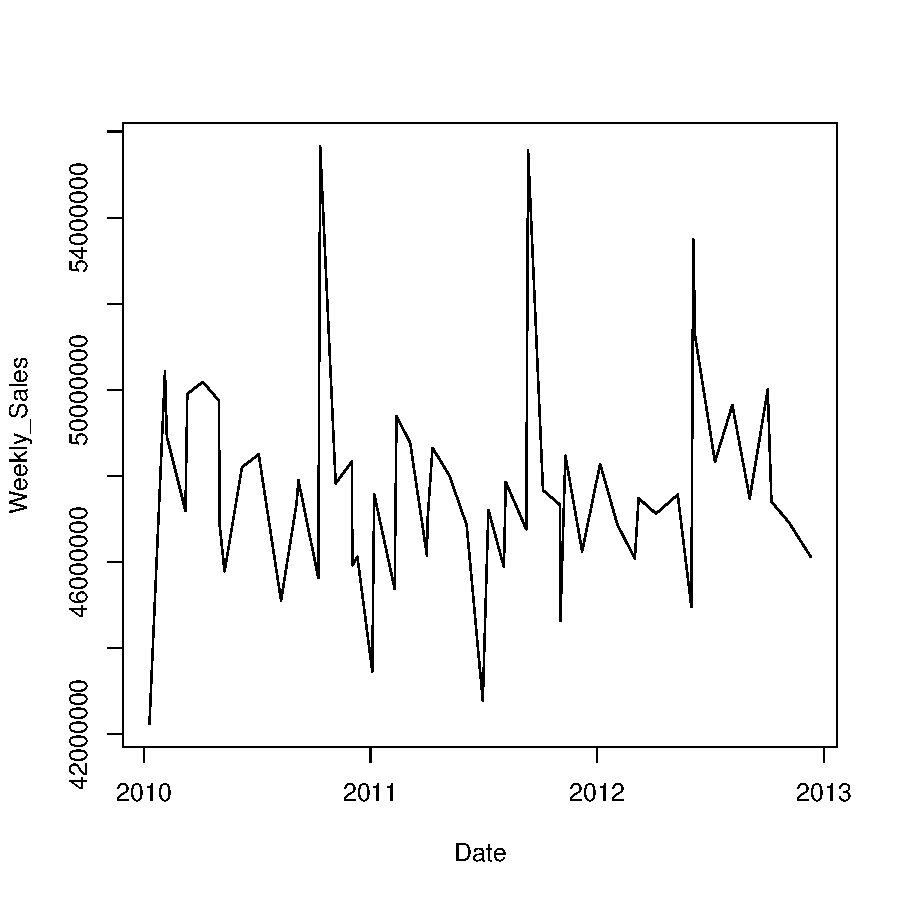
\includegraphics[width=.6\linewidth]{figure/Walmart-Sales-Rnwauto-report-2} 

}


\begin{kframe}\begin{alltt}
\hlkwd{class}\hlstd{(store1)}
\end{alltt}
\begin{verbatim}
## [1] "data.frame"
\end{verbatim}
\begin{alltt}
\hlkwd{str}\hlstd{(store1)}
\end{alltt}
\begin{verbatim}
## 'data.frame':	57 obs. of  2 variables:
##  $ Date        : Date, format: "2010-01-10" "2010-02-04" ...
##  $ Weekly_Sales: num  42239876 50423831 48917484 47194258 49909028 ...
\end{verbatim}
\begin{alltt}
\hlcom{#preparing data for ARIMA model}
\hlkwd{library}\hlstd{(dplyr)}
\hlstd{store_month_year} \hlkwb{<-} \hlkwd{transform}\hlstd{(stores,}\hlkwc{Year} \hlstd{=}\hlkwd{as.numeric}\hlstd{(}\hlkwd{format}\hlstd{(Date,}\hlstr{"%Y"}\hlstd{))}
                                     \hlstd{,}\hlkwc{Month} \hlstd{=}\hlkwd{as.numeric}\hlstd{(}\hlkwd{format}\hlstd{(Date,}\hlstr{"%m"}\hlstd{)))}
\hlstd{store_month_year_filtered} \hlkwb{<-} \hlstd{store_month_year} \hlopt \hlstd{dplyr}\hlopt{::} \hlkwd{select}\hlstd{(Weekly_Sales,Year,Month)}

\hlcom{# rolling up sales at month level}
\hlstd{Walmart_Rolledup} \hlkwb{<-} \hlkwd{aggregate}\hlstd{(Weekly_Sales}\hlopt{~}\hlstd{Year}\hlopt{+}\hlstd{Month,}
                             \hlstd{store_month_year_filtered,sum)}
\hlcom{# sorting in year and month order}
\hlstd{Walmart_sorted} \hlkwb{<-} \hlkwd{arrange}\hlstd{(Walmart_Rolledup,Year,Month)}
\hlcom{# creating a Column with month and year of sale}
\hlstd{Walmart_TS} \hlkwb{<-} \hlkwd{transform}\hlstd{(Walmart_sorted,}
                        \hlkwc{Time_Of_Sale} \hlstd{=} \hlkwd{as.Date}\hlstd{(}\hlkwd{paste}\hlstd{(Year,}\hlstr{"-"}\hlstd{,Month,}\hlstr{"-"}\hlstd{,}\hlnum{1}\hlstd{,}\hlkwc{sep}\hlstd{=}\hlstr{""}\hlstd{),}
                                                             \hlkwc{format}\hlstd{=}\hlstr{"%Y-%m-%d"}\hlstd{))[,}\hlkwd{c}\hlstd{(}\hlnum{4}\hlstd{,}\hlnum{3}\hlstd{)]}

\hlcom{# Build up ARIMA model to forecast last 6 months i.e as in input utilize only till }
\hlcom{# Building ARIMA model}
\hlstd{Walmart_ARIMA} \hlkwb{<-} \hlkwd{auto.arima}\hlstd{(Walmart_TS[}\hlnum{1}\hlopt{:}\hlnum{30}\hlstd{,}\hlnum{2}\hlstd{])}
\hlstd{Walmart_ARIMA} \hlkwb{=} \hlkwd{arima}\hlstd{(Walmart_TS[}\hlnum{1}\hlopt{:}\hlnum{30}\hlstd{,}\hlnum{2}\hlstd{],}\hlkwc{order}\hlstd{=}\hlkwd{c}\hlstd{(}\hlnum{2}\hlstd{,}\hlnum{1}\hlstd{,}\hlnum{2}\hlstd{))}
\hlstd{Forecasted_Sale} \hlkwb{<-} \hlkwd{forecast}\hlstd{(Walmart_ARIMA,}\hlkwc{h}\hlstd{=}\hlnum{6}\hlstd{)}
\hlstd{Forecasted_Sale}
\end{alltt}
\begin{verbatim}
##    Point Forecast    Lo 80     Hi 80     Lo 95     Hi 95
## 31       55283481 11525889  99041072 -11637980 122204942
## 32       77502995 30890120 124115869   6214755 148791234
## 33       83858952 37238984 130478921  12559863 155158042
## 34       77169672 30405443 123933900   5649956 148689388
## 35       79070346 32314786 125825905   7563888 150576804
## 36       79374165 32616364 126131967   7864278 150884052
\end{verbatim}
\begin{alltt}
\hlkwd{jpeg}\hlstd{(}\hlstr{'sales_forecast_6m.jpg'}\hlstd{)}
\hlkwd{plot}\hlstd{(Forecasted_Sale)}
\hlkwd{dev.off}\hlstd{()}
\end{alltt}
\begin{verbatim}
## RStudioGD 
##         2
\end{verbatim}
\begin{alltt}
\hlcom{# 6 months forecast}
\hlstd{Forecasted_Sales} \hlkwb{<-} \hlkwd{as.data.frame}\hlstd{(Forecasted_Sale)}
\hlstd{Forecasted_Sales_6m} \hlkwb{<-} \hlstd{Forecasted_Sales[,}\hlnum{1}\hlstd{]}
\hlkwd{View}\hlstd{(Forecasted_Sales_6m)}
\hlcom{# 6 m actual}
\hlstd{Actual_Sales_6m} \hlkwb{<-} \hlstd{Walmart_TS[}\hlnum{31}\hlopt{:}\hlnum{36}\hlstd{,]}
\hlcom{# concatenating 6 m forecast and actual}
\hlstd{Actual_vs_Forecast_last_6_m} \hlkwb{<-} \hlkwd{cbind}\hlstd{(Forecasted_Sales_6m,Actual_Sales_6m)}
\hlkwd{View}\hlstd{(Actual_vs_Forecast_last_6_m)}
\hlstd{p1}\hlkwb{<-}\hlkwd{ggplot}\hlstd{(Actual_vs_Forecast_last_6_m,} \hlkwd{aes}\hlstd{(Time_Of_Sale, Forecasted_Sales_6m))}\hlopt{+}
  \hlkwd{geom_line}\hlstd{()}\hlopt{+}\hlkwd{ggtitle}\hlstd{(}\hlstr{"Six-Month Sales Forecast"}\hlstd{)}
\hlstd{p1}
\end{alltt}
\end{kframe}

{\centering 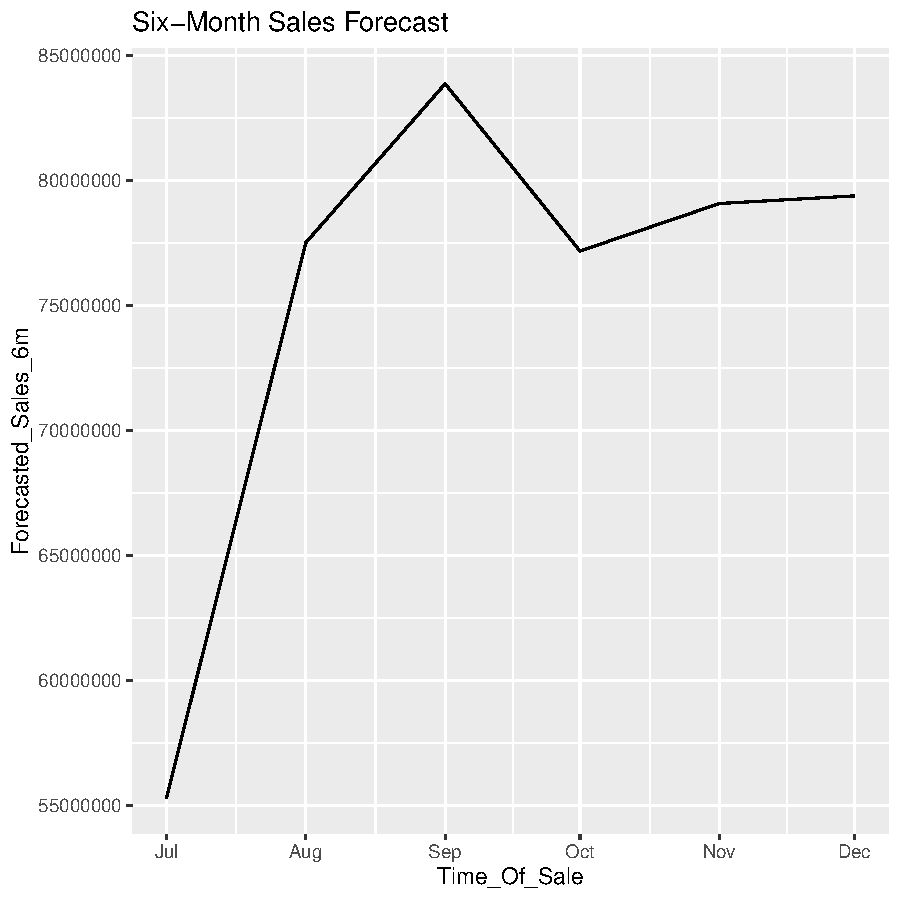
\includegraphics[width=.6\linewidth]{figure/Walmart-Sales-Rnwauto-report-3} 

}


\begin{kframe}\begin{alltt}
\hlstd{p2}\hlkwb{<-}\hlkwd{ggplot}\hlstd{(Actual_vs_Forecast_last_6_m,} \hlkwd{aes}\hlstd{(Time_Of_Sale, Weekly_Sales))}\hlopt{+}
  \hlkwd{geom_line}\hlstd{()}\hlopt{+}\hlkwd{ggtitle}\hlstd{(}\hlstr{"Actual Sales"}\hlstd{)}
\hlstd{p2}
\end{alltt}
\end{kframe}

{\centering 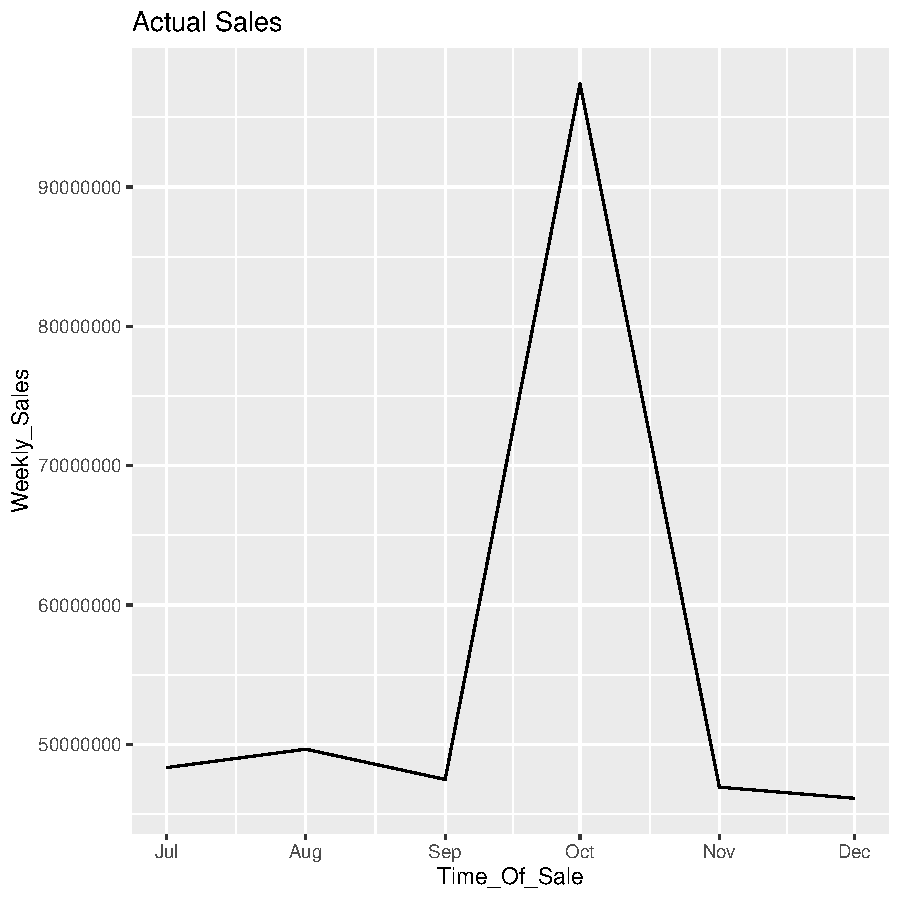
\includegraphics[width=.6\linewidth]{figure/Walmart-Sales-Rnwauto-report-4} 

}


\begin{kframe}\begin{alltt}
\hlkwd{install.packages}\hlstd{(}\hlstr{'patchwork'}\hlstd{)}
\end{alltt}
\begin{verbatim}
## Error in install.packages : Updating loaded packages
\end{verbatim}
\begin{alltt}
\hlkwd{library}\hlstd{(patchwork)}
\hlstd{p1}\hlopt{+}\hlstd{p2}
\end{alltt}
\end{kframe}

{\centering 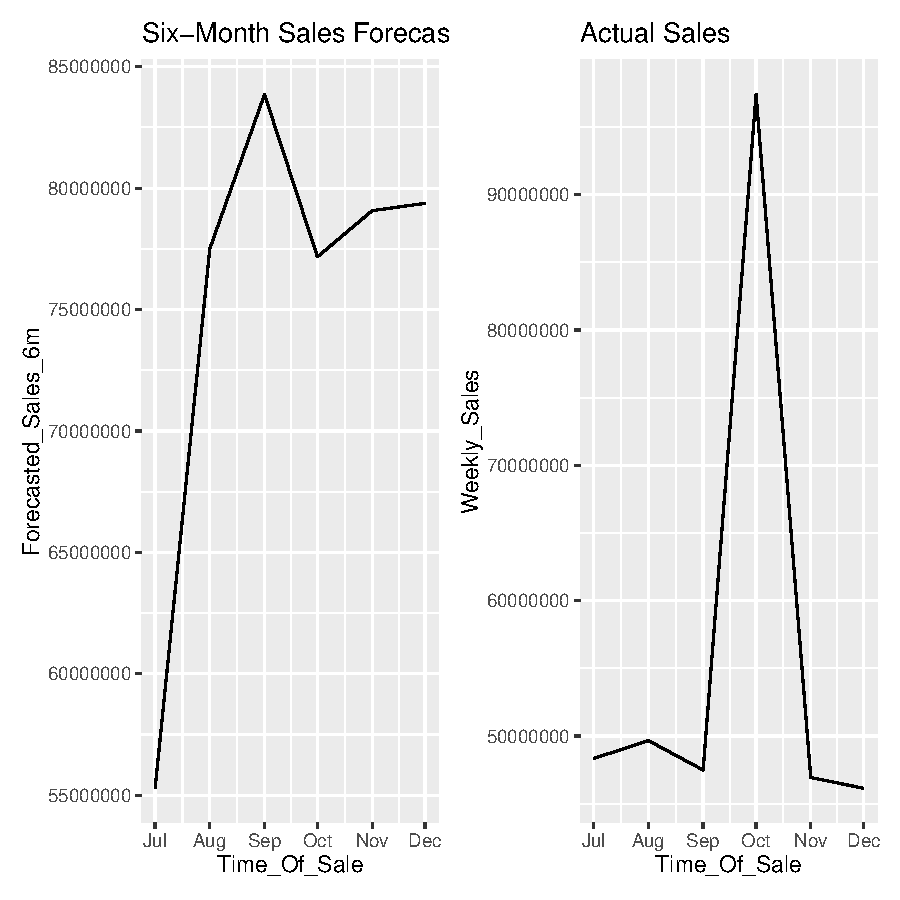
\includegraphics[width=.6\linewidth]{figure/Walmart-Sales-Rnwauto-report-5} 

}


\begin{kframe}\begin{alltt}
\hlstd{Actual_vs_Forecast_last_6_m_deviation} \hlkwb{<-} \hlkwd{transform}\hlstd{(Actual_vs_Forecast_last_6_m,}
                                                 \hlkwc{Errors} \hlstd{=} \hlkwd{abs}\hlstd{(Forecasted_Sales_6m}\hlopt{-}\hlstd{Weekly_Sales)}\hlopt{/}\hlstd{Weekly_Sales)}
\hlstd{MAPE} \hlkwb{<-} \hlkwd{mean}\hlstd{(Actual_vs_Forecast_last_6_m_deviation}\hlopt{$}\hlstd{Errors)}
\hlstd{MAPE}
\end{alltt}
\begin{verbatim}
## [1] 0.5140889
\end{verbatim}
\end{kframe}
\end{knitrout}

The R session information (including the OS info, R version and all
packages used):

\begin{knitrout}
\definecolor{shadecolor}{rgb}{0.969, 0.969, 0.969}\color{fgcolor}\begin{kframe}
\begin{alltt}
\hlkwd{sessionInfo}\hlstd{()}
\end{alltt}
\begin{verbatim}
## R version 4.0.5 (2021-03-31)
## Platform: x86_64-apple-darwin17.0 (64-bit)
## Running under: macOS Big Sur 10.16
## 
## Matrix products: default
## LAPACK: /Library/Frameworks/R.framework/Versions/4.0/Resources/lib/libRlapack.dylib
## 
## locale:
## [1] en_US.UTF-8/en_US.UTF-8/en_US.UTF-8/C/en_US.UTF-8/en_US.UTF-8
## 
## attached base packages:
## [1] stats     graphics  grDevices utils     datasets  methods   base     
## 
## other attached packages:
##  [1] patchwork_1.1.1  forecast_8.15    lmtest_0.9-38    usdm_1.1-18      zoo_1.8-9       
##  [6] raster_3.4-10    sp_1.4-5         plyr_1.8.6       dplyr_1.0.5      lubridate_1.7.10
## [11] ggplot2_3.3.3   
## 
## loaded via a namespace (and not attached):
##  [1] tinytex_0.31      tidyselect_1.1.0  xfun_0.22         purrr_0.3.4      
##  [5] urca_1.3-0        lattice_0.20-41   colorspace_2.0-0  vctrs_0.3.7      
##  [9] generics_0.1.0    htmltools_0.5.1.1 utf8_1.2.1        rlang_0.4.10     
## [13] pillar_1.6.0      glue_1.4.2        withr_2.4.2       DBI_1.1.1        
## [17] TTR_0.24.2        lifecycle_1.0.0   stringr_1.4.0     quantmod_0.4.18  
## [21] timeDate_3043.102 munsell_0.5.0     gtable_0.3.0      evaluate_0.14    
## [25] codetools_0.2-18  knitr_1.33        labeling_0.4.2    tseries_0.10-48  
## [29] parallel_4.0.5    curl_4.3          fansi_0.4.2       highr_0.9        
## [33] xts_0.12.1        Rcpp_1.0.6        scales_1.1.1      farver_2.1.0     
## [37] fracdiff_1.5-1    digest_0.6.27     stringi_1.5.3     grid_4.0.5       
## [41] quadprog_1.5-8    tools_4.0.5       magrittr_2.0.1    tibble_3.1.1     
## [45] crayon_1.4.1      pkgconfig_2.0.3   ellipsis_0.3.1    rmarkdown_2.7    
## [49] assertthat_0.2.1  rstudioapi_0.13   R6_2.5.0          nnet_7.3-15      
## [53] nlme_3.1-152      compiler_4.0.5
\end{verbatim}
\begin{alltt}
\hlkwd{Sys.time}\hlstd{()}
\end{alltt}
\begin{verbatim}
## [1] "2021-06-08 11:01:49 IST"
\end{verbatim}
\end{kframe}
\end{knitrout}


\end{document}
